\documentclass[conference]{IEEEtran}
\IEEEoverridecommandlockouts

\usepackage{cite}
\usepackage{amsmath,amssymb}
\usepackage{algorithmic}
\usepackage{algorithm}
\usepackage{array}
\usepackage{booktabs}
\usepackage{graphicx}
\usepackage{textcomp}
\usepackage{xcolor}
\usepackage{url}
\usepackage{tikz}
\usetikzlibrary{arrows.meta,positioning,calc}
\setlength{\emergencystretch}{1.5em}

\def\BibTeX{{\rm B\kern-.05em{\sc i\kern-.025em b}\kern-.08em
    T\kern-.1667em\lower.7ex\hbox{E}\kern-.125emX}}

\begin{document}

\title{ReachSBOM: A Reachability-Aware Vulnerability Orchestrator for Prioritizing Dependency Vulnerabilities}

\author{\IEEEauthorblockN{Uday Singh, Sujal Rana, and Vivek Kumar}
\IEEEauthorblockA{Department of Information Technology\\
Galgotias College of Engineering and Technology\\
Greater Noida, India}}

\maketitle

\begin{abstract}
Software composition analysis tools report a vulnerability whenever a dependency version matches a known CVE, whether or not the vulnerable code can run in the application. An earlier study reports a false-positive rate of 97.5\% for this kind of version-based matching, and a recent propagation model shows that mainstream SBOM tools cover only the structural stages of vulnerability propagation. This paper presents ReachSBOM, a freely available command-line tool that adds the missing reachability stage. ReachSBOM generates a CycloneDX SBOM with Syft, maps components to advisories from OSV.dev, resolves the vulnerable methods behind each advisory, builds a call graph with Soot, and decides whether each vulnerable method is reachable from application entry points. A small set of framework-aware edge rules models calls that plain static analysis misses, such as plugin instantiation through reflection. A stage-aware risk score combines CVSS severity with reachability status to rank findings. The current version targets Java projects built with Maven. We describe the design and report an evaluation that uses a seeded benchmark of library-usage patterns, the Spring Boot Log4Shell case study from prior work, two binary distributions for Stage 1 and Stage 2 checks, and a corpus of five real Maven projects. The baselines are Syft with Grype, Trivy, and a direct call-site query.
\end{abstract}

\begin{IEEEkeywords}
software supply chain security, SBOM, reachability analysis, call graph, vulnerability prioritization, software composition analysis
\end{IEEEkeywords}

\section{Introduction}
Third-party libraries make up a large share of the code in a modern application, and most of them arrive as transitive dependencies that no developer chose directly. A flaw in any of these libraries reaches every application that ships it. Log4Shell (CVE-2021-44228) showed how far this can go: a single logging library exposed servers across the whole software ecosystem within hours of disclosure~\cite{grgic}.

Software Bills of Materials (SBOMs) and software composition analysis (SCA) tools were introduced to give organizations visibility into this exposure. They list the components of an application and match each name and version against vulnerability databases such as the National Vulnerability Database (NVD)~\cite{nvd} and OSV~\cite{osv}. The match answers one question, whether a vulnerable version is present. It does not answer whether the vulnerable code can ever execute. Zhou et al.\ measured the cost of this gap and report a false-positive rate of 97.5\% for version-based vulnerability scanning, a figure that did not drop after the input to the scanners was made more accurate~\cite{zhou},~\cite{grgic}. Developers who receive hundreds of such alerts either patch indiscriminately or stop reading them.

Grgic et al.\ describe the problem as a missing step in a four-stage propagation model: structural exposure, vulnerable class presence, code reachability, and taint path confirmation~\cite{grgic}. Evaluating Syft, Trivy, Grype, and cdxgen on Apache Solr 8.11.0, Spring Boot 2.5.0, and Ghidra 10.0.4, they found that the tools support the first two stages and cannot establish the third or fourth. They obtained Stage~3 and Stage~4 evidence only by running separate program-analysis tools, CodeQL and Semgrep, by hand. Their paper ends by calling for tools that capture propagation-stage information.

This paper takes up that call. We present ReachSBOM, an automated pipeline that takes a repository as input and produces a vulnerability report ranked by reachability. The pipeline connects SBOM generation, advisory mapping, call-graph construction, and risk scoring, so that Stage~3 evidence is produced in the same run as the SBOM instead of in a separate manual analysis.

The contributions of this paper are as follows.
\begin{enumerate}
\item A freely available command-line tool that implements Stages~1 to~3 of the propagation model in a single run, for Java projects built with Maven.
\item A method for resolving the vulnerable methods behind an advisory and deciding their reachability with a call graph extended by framework-aware edge rules.
\item A stage-aware risk score and a report that ranks findings by reachability.
\item An evaluation with a seeded benchmark, a replication of the Log4Shell case study of~\cite{grgic}, and a corpus of five real Maven projects.
\end{enumerate}

The rest of the paper is organized as follows. Section~\ref{sec:background} gives background, Section~\ref{sec:related} reviews related work, Sections~\ref{sec:design} and~\ref{sec:impl} describe the design and implementation, Section~\ref{sec:eval} defines the evaluation, Section~\ref{sec:results} reports results, and Sections~\ref{sec:discussion} and~\ref{sec:conclusion} discuss limitations and conclude.

\section{Background}\label{sec:background}

\subsection{SBOMs and Software Composition Analysis}
An SBOM is a machine-readable inventory of the components in a software product. A typical entry records a name, a version, a package URL (purl), hashes, and the dependency relationships between components. CycloneDX~\cite{cyclonedx} and SPDX are the two dominant formats. Generators such as Syft~\cite{syft} and cdxgen read build metadata, lock files, container layers, or compiled artifacts and emit this inventory. Their output depends on the input they receive: a manifest, a resolved dependency tree, and a packaged distribution can yield different component lists for the same project~\cite{grgic},~\cite{balliu}.

SCA tools consume the inventory and match each component against advisory databases. The NVD~\cite{nvd} identifies affected products with CPE names, while OSV~\cite{osv} expresses affected versions as ranges per package ecosystem. Severity is usually taken from the Common Vulnerability Scoring System (CVSS)~\cite{cvss}. CVSS describes the intrinsic severity of a flaw. It carries no information about the application that uses the vulnerable library.

\subsection{The Four-Stage Propagation Model}
Grgic et al.\ split the path from a vulnerable dependency to a possible exploit into four stages~\cite{grgic}. Each stage needs stronger evidence than the previous one (Table~\ref{tab:stages}).

\begin{table}[t]
\caption{Stages of the propagation model of~\cite{grgic}.}
\label{tab:stages}
\centering
\footnotesize
\renewcommand{\arraystretch}{1.15}
\setlength{\tabcolsep}{2.5pt}
\begin{tabular}{@{}p{0.9in}p{1.15in}p{1.2in}@{}}
\toprule
Stage & Question answered & Evidence required \\
\midrule
1. Structural exposure & Is the vulnerable component present? & Component and version in the dependency tree \\
2. Vulnerable class presence & Does the vulnerable class exist on the classpath? & Class entry in the artifact \\
3. Code reachability & Can application code reach the vulnerable method? & Call path from an entry point \\
4. Taint path confirmation & Can attacker-controlled data reach the vulnerable sink? & Source-to-sink data flow \\
\bottomrule
\end{tabular}
\end{table}

SBOM generators and version-matching scanners operate on the first row and partly on the second. The remaining rows are program-analysis problems.

\subsection{Call Graphs and Reachability}
A call graph has one node per method and an edge for each possible call. For object-oriented code the edges of virtual calls must be approximated. Class hierarchy analysis (CHA)~\cite{cha} adds an edge to every override that is type-compatible with the receiver's declared type. Rapid type analysis (RTA)~\cite{rta} keeps only overrides of classes that the program instantiates. Points-to based construction, such as the SPARK framework in Soot~\cite{soot},~\cite{spark}, tracks which objects can reach each receiver and gives the most precise graphs at a higher cost.

Reachability of a method is then a graph query: the method is reachable if a path leads to it from an entry point. The answer is only as good as the graph. Reflection, dynamic proxies, dependency injection, and serialization create calls that are invisible in the bytecode, and an unsound graph turns these cases into false negatives, which is the more dangerous error in a security setting.

\section{Related Work}\label{sec:related}
Several studies examine how vulnerabilities spread through dependency structures. Liu et al.\ analyze propagation and its evolution in npm dependency trees and expose the difficulty of resolving dependencies exactly~\cite{liu}. Ruan et al.\ propose a propagation-based impact assessment with a scoring scheme for whole ecosystems~\cite{ruan}. Xia et al.\ unify SBOM and SCA data in a graph and gain visibility into propagation, but the graph does not record whether vulnerable code is invoked, so false positives remain~\cite{xia}.

A second group of studies measures the quality of SBOM-based management. Balliu et al.\ describe the challenges of producing accurate SBOMs for Java~\cite{balliu}. Zhou et al.\ evaluate SBOM-based vulnerability management empirically and name reachability analysis as a requirement that scanners do not meet~\cite{zhou}. Tesson et al.\ argue that current SBOM techniques cannot trace dependencies from source code to the service level and therefore cannot support operational impact analysis~\cite{tesson}. Grgic et al.\ place these observations in a stage model and show that the evaluated SBOM tools stop after Stage~2~\cite{grgic}.

A third group builds reachability analyses. Patel et al.\ show that code reachability information improves the precision of vulnerability triage~\cite{patel}. ReachCheck~\cite{reachcheck} constructs library-aware call graphs compositionally for use inside IDEs, and a study published in \emph{Computers \& Security} assesses third-party library vulnerabilities through reachability~\cite{cose}.

These lines of work leave a practical gap. Measurement studies~\cite{grgic},~\cite{zhou} diagnose the limitation, graph-based work~\cite{xia},~\cite{ruan} improves visibility without invocation information, and reachability analyses~\cite{reachcheck}--\cite{patel} are not connected to SBOM generation and advisory mapping. ReachSBOM connects the pieces in one command-line tool, adds framework-aware edge rules, and ranks findings by reachability.

\section{ReachSBOM Design}\label{sec:design}

\subsection{Overview}
ReachSBOM takes a Java project, given as a path to the project folder, and runs four stages in sequence (Fig.~\ref{fig:pipeline}). Each stage writes its result to a JSON file in the output folder, so later stages can read earlier evidence and the final report can trace every verdict back to its source.

\begin{figure*}[t]
\centering
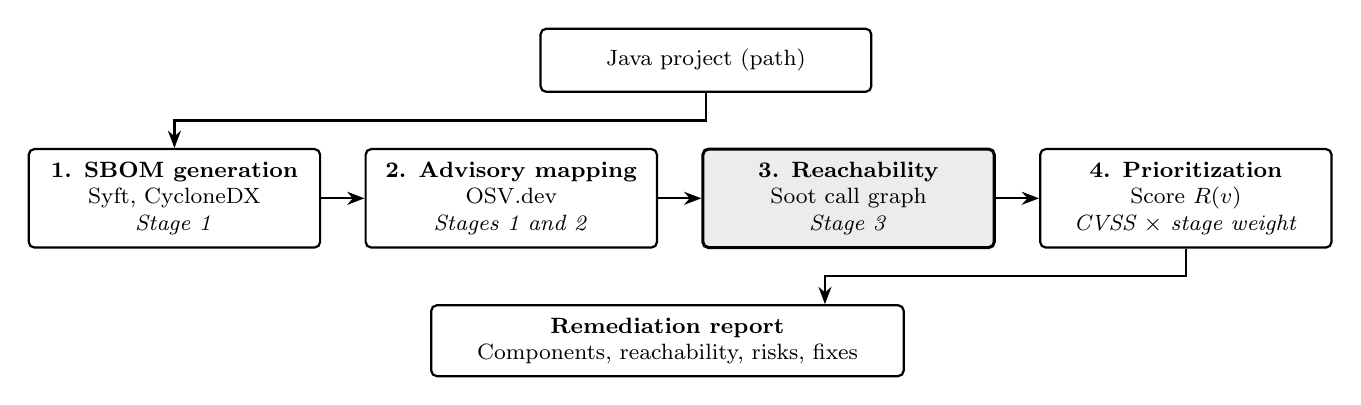
\begin{tikzpicture}[
  font=\footnotesize,
  box/.style={draw, rounded corners=2pt, minimum width=3.7cm, minimum height=1.25cm, align=center, thick},
  main/.style={box, fill=gray!15, line width=1.1pt},
  arr/.style={-{Stealth[length=2.2mm]}, thick}
]
\node[box, minimum width=4.2cm, minimum height=0.8cm] (in) {Java project (path)};
\node[box, below=0.7cm of in, xshift=-6.75cm] (s1) {\textbf{1. SBOM generation}\\Syft, CycloneDX\\\textit{Stage 1}};
\node[box, right=0.55cm of s1] (s2) {\textbf{2. Advisory mapping}\\OSV.dev\\\textit{Stages 1 and 2}};
\node[main, right=0.55cm of s2] (s3) {\textbf{3. Reachability}\\Soot call graph\\\textit{Stage 3}};
\node[box, right=0.55cm of s3] (s4) {\textbf{4. Prioritization}\\Score $R(v)$\\\textit{CVSS $\times$ stage weight}};
\node[box, below=0.7cm of s3, xshift=-2.3cm, minimum width=6cm, minimum height=0.9cm] (rep) {\textbf{Remediation report}\\Components, reachability, risks, fixes};
\draw[arr] (in.south) -- ++(0,-0.35) -| (s1.north);
\draw[arr] (s1) -- (s2);
\draw[arr] (s2) -- (s3);
\draw[arr] (s3) -- (s4);
\draw[arr] (s4.south) -- ++(0,-0.35) -| ([xshift=2.0cm]rep.north);
\end{tikzpicture}
\caption{ReachSBOM pipeline. Stage~3 (shaded) supplies the evidence that SBOM generators and version-matching scanners cannot produce.}
\label{fig:pipeline}
\end{figure*}

\subsection{SBOM Generation}
The first stage resolves the dependency tree and emits a CycloneDX SBOM with Syft. Because the output of a generator depends on its input~\cite{grgic}, ReachSBOM runs Syft on the resolved Maven dependency tree and the runtime classpath instead of on the manifest alone, and it falls back to scanning the packaged JAR files when no build file is available. Components are identified by package URL.

\subsection{Advisory Mapping and Vulnerable Symbols}
For each component the second stage queries OSV.dev by package URL and version. Records that describe the same flaw are merged through their aliases (CVE and GHSA identifiers), and the affected version ranges are checked against the resolved version. The CVSS vector in the advisory supplies the severity value $S(v)$.

Reachability needs a target method, and advisories rarely name one. ReachSBOM therefore reads vulnerable symbols from a symbol file that lists, for each advisory, the classes and methods that contain the flaw. Entries for the libraries in the evaluation are written by hand from the fix commit and the advisory text, and each entry cites its source. A vulnerability with no entry falls back to component-level reachability, described below.

The stage also performs the Stage~2 check. It opens the JAR that carries the component and tests whether the class entries that contain the vulnerable symbols exist and have not been removed.

\subsection{Reachability Analysis}
The third stage decides whether application code can reach a vulnerable method. It has four parts.

\emph{Entry points.} The analysis starts from the main methods of the application, the request-handling methods of servlets, and the handler methods that web frameworks register through annotations such as Spring's request mappings. For libraries, all public methods serve as entry points.

\emph{Call graph.} Soot builds a whole-program call graph over application classes and dependency JARs. The default algorithm is RTA for speed, and class hierarchy analysis is used as an ablation.

\emph{Framework-aware edges.} Static call graphs miss calls that frameworks make on behalf of the application. Log4j~2, for example, resolves lookups through a plugin registry, so application code never names the lookup class that handles a logged string. ReachSBOM therefore reads a set of declarative edge rules. A rule states that a call to a given set of methods implies a call to another set, for example from the public logging methods to the lookup dispatch of the interpolator. Rules are plain files kept next to the symbol map, and each carries the advisory or documentation that justifies it. Calls through reflection with a constant class name are resolved directly. Calls with a non-constant target are recorded as unresolved so that they influence the verdict.

\emph{Verdict.} For each vulnerable symbol the stage runs a path query and assigns one of the statuses in Table~\ref{tab:status}. A path that depends on an unresolved reflective call is reported as possibly reachable instead of reachable.

\begin{table}[t]
\caption{Reachability statuses and the propagation stage each corresponds to.}
\label{tab:status}
\centering
\footnotesize
\renewcommand{\arraystretch}{1.15}
\setlength{\tabcolsep}{2.5pt}
\begin{tabular}{@{}p{0.95in}p{1.95in}c@{}}
\toprule
Status & Meaning & Stage \\
\midrule
Present & Component in dependency tree & 1 \\
Class present & Vulnerable class found in the artifact, no path from an entry point & 2 \\
Possibly reachable & Path exists only through an unresolved dynamic call, or only the component level could be checked & 3 \\
Reachable & Path from an entry point to the vulnerable method & 3 \\
Taint confirmed & Attacker-controlled source reaches the sink & 4 \\
\bottomrule
\end{tabular}
\end{table}

Algorithm~\ref{alg:verdict} summarizes the verdict computation.

\begin{algorithm}[t]
\caption{Reachability verdict for one advisory}
\label{alg:verdict}
\small
\begin{algorithmic}[1]
\REQUIRE call graph $G$, entry points $E$, vulnerable symbols $M$, edge rules $R$
\STATE $G \leftarrow \mathrm{apply}(R, G)$
\IF{$M = \emptyset$}
  \RETURN \textsc{PossiblyReachable} if any application method reaches the artifact, else \textsc{ClassPresent}
\ENDIF
\FOR{each $m \in M$}
  \IF{$m \in G$ and a path $e \rightarrow m$ exists with $e \in E$}
    \IF{the path contains an unresolved dynamic call}
      \STATE $status \leftarrow$ \textsc{PossiblyReachable}
    \ELSE
      \STATE $status \leftarrow$ \textsc{Reachable}
    \ENDIF
  \ENDIF
\ENDFOR
\RETURN the strongest status over $M$, or \textsc{ClassPresent} if no $m$ has a path
\end{algorithmic}
\end{algorithm}

Stage~4 is outside the scope of the current version. The report keeps the reachable sinks in a form that a taint-analysis tool such as Semgrep or CodeQL, as used in~\cite{grgic}, can consume later.

\subsection{Stage-Aware Risk Score}
The fourth stage ranks findings. For a vulnerability $v$ with CVSS base score $S(v)$ and reachability status $s(v)$, the score is
\begin{equation}
R(v) = \frac{S(v)}{10}\, w\bigl(s(v)\bigr)
\end{equation}
where $w$ is a weight that grows with the stage: 0.2 for Present, 0.4 for Class present, 0.6 for Possibly reachable, 0.8 for Reachable, and 1.0, reserved for Taint confirmed. The weights are initial values and are checked against the benchmark described in Section~\ref{sec:eval}. Because the weight grows with the stage, a reachable medium-severity flaw can outrank an unreachable critical one, which is the intended behavior.

\subsection{Remediation Report}
The report lists each finding with the component, the advisory identifiers, the CVSS score, the reachability status, the call path that supports it, the risk score, and the lowest fixed version listed in the advisory. It is written as a JSON file and as a plain-text summary for the terminal.

\section{Implementation}\label{sec:impl}
ReachSBOM is a command-line tool. The orchestrator is written in Python. It calls Syft as an external process, queries the OSV.dev API, and calls a Java module for the reachability stage. The Java module is built on Soot, receives the resolved classpath and the list of vulnerable symbols, and returns verdicts and supporting paths as JSON. Responses from OSV.dev are cached by package URL and version. Symbol files and edge rules are plain files in the repository and are loaded at start-up, so a new rule can be added without changing code. The tool is freely available and can be run by anyone on a Java project with a Maven build.

\section{Evaluation Design}\label{sec:eval}

\subsection{Research Questions and Hypotheses}
The evaluation addresses four questions.
\begin{itemize}
\item \textbf{RQ1:} How accurately does ReachSBOM classify the reachability of vulnerable methods compared with SBOM-only scanning and with direct-call queries?
\item \textbf{RQ2:} How much do framework-aware edge rules and the choice of call-graph algorithm change the verdicts?
\item \textbf{RQ3:} By how much does reachability filtering reduce the number of alerts on real projects, and how well does the risk score rank findings that are truly reachable?
\item \textbf{RQ4:} What time and memory overhead does the analysis add to SBOM generation and scanning?
\end{itemize}

We state two hypotheses in advance. \textbf{H1:} version-based scanners report the same findings for every application in the seeded benchmark, independent of how the vulnerable library is used, as observed in~\cite{grgic}. \textbf{H2:} with framework-aware edge rules, ReachSBOM classifies the Log4Shell projects as reachable or possibly reachable wherever the application contains a logging call, even though a direct-call query for \texttt{JndiLookup.lookup()} returns no match.

\subsection{Benchmarks}
\emph{Set~A} is a seeded benchmark with known ground truth. Each application depends on a vulnerable library and uses it in one of ten patterns (Table~\ref{tab:patterns}). The patterns are instantiated for three libraries: log4j-core 2.14.1 (CVE-2021-44228), commons-text 1.9 (CVE-2022-42889), and snakeyaml 1.33 (CVE-2022-1471). This gives 30 applications.

\begin{table}[t]
\caption{Seeded usage patterns in benchmark Set~A.}
\label{tab:patterns}
\centering
\footnotesize
\renewcommand{\arraystretch}{1.1}
\begin{tabular}{@{}l p{1.85in} p{0.85in}@{}}
\toprule
Pattern & Use of the vulnerable library & Expected status \\
\midrule
P1 & Declared as a dependency, never referenced & Present \\
P2 & Class on the classpath, never referenced & Class present \\
P3 & Direct call to the vulnerable method & Reachable \\
P4 & Call through a chain of three helper methods & Reachable \\
P5 & Call through an interface or virtual dispatch & Reachable \\
P6 & Reflection with a constant class name & Reachable \\
P7 & Reflection with a computed class name & Possibly reachable \\
P8 & Call only in a method that no entry point reaches & Class present \\
P9 & Call only in test sources & Class present \\
P10 & Call made by a framework on behalf of the application & Reachable \\
\bottomrule
\end{tabular}
\end{table}

\emph{Set~B} contains the Spring Boot 2.5.0 Log4Shell case study and two binary distributions from prior work, Apache Solr 8.11.0 with log4j-core 2.14.1 and Ghidra 10.0.4 with log4j-core 2.12.1. ReachSBOM analyzes the Maven case study end to end. The binary distributions are used for Stage~1 and Stage~2 checks only, because the current prototype requires a Maven build to construct an application call graph. The Stage~1 to Stage~3 outcomes published in~\cite{grgic} serve as the reference.

\emph{Set~C} is a corpus of five publicly hosted Spring Guides Maven projects that build successfully and carry at least one dependency with a published advisory. The projects cover a plain Maven application and four Spring Boot applications, with 3 to 48 resolved JARs. Because no ground truth exists for these projects, one reviewer triaged the ten highest-ranked findings by inspecting the reported call paths and the source code. A finding counted as confirmed only when the path started at an application entry point and ended at the vulnerable method. The single-reviewer protocol does not support an agreement statistic.

\subsection{Baselines and Ablations}
The baselines are Syft with Grype and Trivy, two of the tools evaluated in~\cite{grgic}. A direct call-site query over all compiled classes, including tests, represents the source-level query approach of~\cite{grgic}; it reports a finding when bytecode contains a call to the vulnerable method, independent of whether an entry point reaches the call. Two ablations of ReachSBOM isolate its components: one without framework-aware edge rules, and one with class hierarchy analysis in place of RTA.

\subsection{Metrics and Procedure}
On Set~A we report per-pattern accuracy and the precision, recall, and F1 score of the reachable class, treating Reachable and Possibly reachable as positive. On Set~C we report the false-positive reduction rate,
\begin{equation}
\mathrm{FPRR} = 1 - \frac{N_{\text{kept}}}{N_{\text{raised}}},
\end{equation}
where $N_{\text{kept}}$ is the number of findings kept as reachable or possibly reachable and $N_{\text{raised}}$ is the number raised by SBOM-only scanning. We also report the precision at $k$ of the risk ranking, defined as the share of the $k$ highest-ranked findings that the reviewer confirms as reachable. For RQ4 we measure wall-clock time and peak memory per project on the same machine. We report the median across Set~C for the SBOM and advisory stages, and amortize the call-graph cost over the five-project batch.

\section{Results}\label{sec:results}

\subsection{Reachability Accuracy on Set~A (RQ1, RQ2)}
Table~\ref{tab:seta} reports precision, recall, and F1 score of the reachable class on the 30 seeded applications for each approach and for the two ablations.

\begin{table}[t]
\caption{Reachability classification on benchmark Set~A.}
\label{tab:seta}
\centering
\footnotesize
\renewcommand{\arraystretch}{1.1}
\setlength{\tabcolsep}{3pt}
\begin{tabular}{@{}lccc@{}}
\toprule
Approach & Precision & Recall & F1 \\
\midrule
Syft + Grype & 0.600 & 1.000 & 0.750 \\
Trivy & 0.667 & 1.000 & 0.800 \\
Direct call sites & 0.647 & 0.611 & 0.629 \\
No edge rules & 1.000 & 0.833 & 0.909 \\
CHA & 1.000 & 1.000 & 1.000 \\
RTA + edge rules & 1.000 & 1.000 & 1.000 \\
\bottomrule
\end{tabular}
\end{table}

The version-matching baselines report the target Log4Shell, Text4Shell, or SnakeYAML advisory in all 30 applications, so recall is 1.0 and precision is bounded by the 12 negative patterns. Grype reports all 30, while Trivy skips the three provided-dependency cases. The direct call-site query detects 17 applications, including the six cases in P8 and P9 where the call exists in bytecode but no entry point reaches it; its precision falls to 0.647 and recall to 0.611. ReachSBOM with RTA and edge rules classifies all 30 patterns correctly. Removing edge rules loses P10 for all three libraries, because the framework dispatch never appears in the bytecode. CHA produces the same Set~A verdicts, but the Spring Boot ablation below shows the cost of its broader dispatch.

\subsection{Log4Shell Replication on Set~B (RQ1)}
Table~\ref{tab:setb} compares the stage outcomes reported in~\cite{grgic} with the status that ReachSBOM assigns to the same projects.

\begin{table}[t]
\caption{Stage outcomes in~\cite{grgic} and ReachSBOM status for the Log4Shell projects.}
\label{tab:setb}
\centering
\scriptsize
\setlength{\tabcolsep}{3pt}
\renewcommand{\arraystretch}{1.1}
\begin{tabular}{@{}lcccc@{}}
\toprule
Project & Stage 1 & Stage 2 & Stage 3 & ReachSBOM \\
\midrule
Apache Solr 8.11.0 & Confirmed & Confirmed & No & Stage 2 \\
Spring Boot 2.5.0 & Confirmed & Confirmed & No & Reachable \\
Ghidra 10.0.4 & Confirmed & Confirmed & No & Stage 2 \\
\bottomrule
\end{tabular}
\end{table}

On \texttt{spring-log4shell}, both RTA and CHA return \textsc{Reachable}. On \texttt{spring-nolog}, RTA returns \textsc{ClassPresent} and CHA returns \textsc{Reachable}. The CHA path runs from Spring Boot startup logging through the log4j interceptor chain to \texttt{JndiLookup}, even though the application never logs request data. This is the false positive that the RTA instance filter and the application-scope edge rule remove. Solr and Ghidra reach Stage~2: the JARs contain \texttt{JndiLookup}, and Grype reports the target advisory in both SBOMs. Stage~3 is not analyzed because neither distribution is a Maven project.

\subsection{Alert Reduction and Ranking on Set~C (RQ3)}
Table~\ref{tab:setc} summarizes the effect of reachability filtering on the five-project corpus.

\begin{table}[t]
\caption{Alert reduction and ranking quality on benchmark Set~C.}
\label{tab:setc}
\centering
\footnotesize
\renewcommand{\arraystretch}{1.1}
\begin{tabular}{@{}p{2.35in}r@{}}
\toprule
Measure & Value \\
\midrule
Projects in the corpus & 5 \\
SBOM-only findings & 449 \\
Kept as reachable & 4 \\
Alert reduction rate & 99.1\% \\
Precision at 10 & 0.40 \\
Reviewer agreement & Single reviewer \\
\bottomrule
\end{tabular}
\end{table}

All four reachable Log4Shell findings occupy the top four ranks. The next six ranks are component-level advisories with no symbol map, so they are not confirmed; precision at 10 is therefore 0.40. The 99.1\% reduction is a filtering rate, not an independent false-positive estimate: 445 of 449 advisories are never promoted to a reachable method, and the four promoted findings are the ones a reviewer can act on first. The no-log JPA project keeps log4j-core at \textsc{ClassPresent}, which is correct for the seeded target but still a component-level alert.

\subsection{Overhead (RQ4)}
Table~\ref{tab:overhead} lists the median cost of each stage.

\begin{table}[t]
\caption{Per-stage cost on Set~C.}
\label{tab:overhead}
\centering
\footnotesize
\renewcommand{\arraystretch}{1.1}
\setlength{\tabcolsep}{3pt}
\begin{tabular}{@{}lcc@{}}
\toprule
Stage & Median time (s) & Peak memory (MB) \\
\midrule
SBOM generation & 2.25 & 194 \\
Advisory mapping & 1.21 & 29 \\
Call graph and reachability & 20.6 & 3059 \\
Scoring and report & 0.06 & 16 \\
\bottomrule
\end{tabular}
\end{table}

The call graph dominates cost. The five-project batch needs 103~s of wall time and 3.0~GB of peak resident memory, or about 20.6~s per project when amortized. SBOM generation and advisory mapping are cache-friendly; the OSV cache reduced advisory mapping to about 1.2~s per project. The 3~GB peak is the main practical limit and is caused by holding the whole Soot scene for a Spring Boot application. A per-project run uses less memory but repeats the graph construction.

\section{Discussion and Limitations}\label{sec:discussion}
The verdicts of ReachSBOM are only as sound as its call graph. Static analysis over-approximates virtual dispatch and under-approximates reflection, dependency injection, and runtime configuration. The framework-aware rules reduce the second problem for the frameworks they cover and do nothing for the rest, so the rule set needs continued maintenance, and each rule needs a reference that a reviewer can check. A Possibly reachable verdict is meant to keep such cases visible instead of silently dropping them.

Symbol resolution is the second limit. Advisories rarely name vulnerable methods, and a method list taken from a fix commit can include refactoring changes that are unrelated to the flaw. A wrong symbol list yields a wrong verdict, so the report shows the symbols used. Where no symbol can be found the pipeline falls back to component-level reachability, which is weaker than the method-level verdict.

Reachability is also not exploitability. A reachable method still needs attacker-controlled input and a suitable configuration before it can be exploited, which is why Stage~4 exists in the model of~\cite{grgic} and why ReachSBOM leaves it as a plug-in interface in this version.

The current prototype targets Java projects built with Maven. Soot does not cover JavaScript or Python, and results may not carry over to those ecosystems. Set~A is synthetic, and Set~C depends on a single reviewer, so the conclusions drawn from them are bounded by the choice of libraries, patterns, and reviewer judgment. The five Set~C projects are all Spring Guides, which limits coverage of build layouts and frameworks.

\section{Conclusion and Future Work}\label{sec:conclusion}
Version-based matching tells developers which vulnerable components they ship, and it cannot tell them which ones can run. Building on the propagation model of Grgic et al.~\cite{grgic}, ReachSBOM connects SBOM generation, advisory mapping, and call-graph reachability in one command-line tool, adds framework-aware edge rules, and ranks findings with a stage-aware score. The evaluation compares it with the tools studied in~\cite{grgic} on a seeded benchmark, on the Log4Shell projects, and on five real Maven projects. Future work includes Stage~4 taint confirmation and reachability analysis for other ecosystems such as JavaScript and Python.

\emph{Data availability.} The source code, symbol files, edge rules, benchmark applications, and result tables are available at \url{https://github.com/Sran012/reachsbom}.

\begin{thebibliography}{1}
\bibitem{grgic} L.~Grgic, L.~Maksimovic, and P.~Laskov, ``Propagation model for SSC attacks: Why SBOM (tools) don't tell the whole truth,'' University of Liechtenstein, 2026.
\bibitem{zhou} L.~Zhou, M.~Dacier, and C.~Konstantinou, ``A reality check on SBOM-based vulnerability management: An empirical study and a path forward,'' arXiv:2511.20313, 2025.
\bibitem{liu} C.~Liu \emph{et al.}, ``Demystifying the vulnerability propagation and its evolution via dependency trees in the NPM ecosystem,'' in \emph{Proc. 44th Int. Conf. Software Engineering (ICSE)}, 2022.
\bibitem{reachcheck} C.~Wang \emph{et al.}, ``ReachCheck: Compositional library-aware call graph reachability analysis in the IDEs,'' \emph{ACM Trans. Softw. Eng. Methodol.}, 2026, doi: 10.1145/3767166.
\bibitem{cose} ``Impact assessment of third-party library vulnerabilities through vulnerability reachability analysis,'' \emph{Computers \& Security}, vol.~157, Art.~no.~104546, 2025, doi: 10.1016/j.cose.2025.104546.
\bibitem{patel} H.~Patel, A.~Snit, and M.~Polychronakis, ``Supply chain reaction: Enhancing the precision of vulnerability triage using code reachability information,'' in \emph{Proc. IEEE Annu. Computer Security Applications Conf. (ACSAC)}, 2025, pp.~92--107.
\bibitem{balliu} M.~Balliu \emph{et al.}, ``Challenges of producing software bill of materials for Java,'' \emph{IEEE Security \& Privacy}, vol.~21, pp.~12--23, 2023.
\bibitem{xia} H.~Xia, J.~Gluck, S.~Simsek, D.~S.~Medina, and D.~Starobinski, ``VDGraph: A graph-theoretic approach to unlock insights from SBOM and SCA data,'' arXiv:2507.20502, 2025.
\bibitem{tesson} L.~Tesson, J.~E.~Hachem, P.~Guillou, and J.~Buisson, ``Towards system-of-systems bill of material solution for vulnerability operational impact analysis,'' in \emph{Proc. IEEE Int. Conf. Trust, Security and Privacy in Computing and Communications (TrustCom)}, 2025.
\bibitem{nvd} National Institute of Standards and Technology, ``National Vulnerability Database (NVD).'' [Online]. Available: https://nvd.nist.gov
\bibitem{osv} Google, ``OSV: Open source vulnerabilities.'' [Online]. Available: https://osv.dev
\bibitem{ruan} B.~Ruan \emph{et al.}, ``Propagation-based vulnerability impact assessment for software supply chains,'' arXiv:2506.01342, 2025.
\bibitem{soot} R.~Vall\'ee-Rai, P.~Co, E.~Gagnon, L.~Hendren, P.~Lam, and V.~Sundaresan, ``Soot: A Java bytecode optimization framework,'' in \emph{Proc. CASCON}, 1999.
\bibitem{cha} J.~Dean, D.~Grove, and C.~Chambers, ``Optimization of object-oriented programs using static class hierarchy analysis,'' in \emph{Proc. ECOOP}, 1995.
\bibitem{rta} D.~F.~Bacon and P.~F.~Sweeney, ``Fast static analysis of C++ virtual function calls,'' in \emph{Proc. OOPSLA}, 1996.
\bibitem{spark} O.~Lhot\'ak and L.~Hendren, ``Scaling Java points-to analysis using SPARK,'' in \emph{Proc. Int. Conf. Compiler Construction (CC)}, 2003.
\bibitem{cvss} Forum of Incident Response and Security Teams, ``Common Vulnerability Scoring System v3.1: Specification document.'' [Online]. Available: https://www.first.org/cvss
\bibitem{cyclonedx} OWASP Foundation, ``CycloneDX bill of materials specification.'' [Online]. Available: https://cyclonedx.org
\bibitem{syft} Anchore, ``Syft: SBOM generator.'' [Online]. Available: https://github.com/anchore/syft
\end{thebibliography}

\end{document}
